\textbf{Please explain your filled-in code with a snapshot of those lines of code. List formulas you have used for that part of code.}\\
The code provided in Fig. (\ref{fig:MotionEst.}) is used for motion prediction and proposal generation. The code is calculating a rigid-body transformation between the two feature points, P and Q, in their respective frames (2 different frames). The steps undertaken can be shown below:
\begin{enumerate}
    \item Extracting the x-y coordinates of P and Q feature points, where a feature point can be understood as a landmark in an environment and can be used for tasks like motion estimation or object recognition to provide properties of a scene
    \begin{align*}
        P_x &= P(:,1) \\
        P_y &= P(:,2) \\
        Q_x &= Q(:,1) \\
        Q_y &= Q(:,2)
    \end{align*}
    \begin{enumerate}
        \item P and Q are existing matrices defined in the code above representing matched feature points in two frames, where P and Q are [n x 2] matrices.  
        \item P contains the feature points in the first frame, and Q contains the feature points in the second frame
        \item $P_x$, $P_y$ extract the x and y coordinates from the first frame, while $Q_x$ and $Q_y$ extract the x and y coordinates from the second frame
    \end{enumerate}
    \item Calculating the Centroid (mean) of the feature points for both frames
    \begin{align}
        \bar{P} &= \left[ \bar{P}_x, \bar{P}_y \right] \\
        \bar{Q} &= \left[ \bar{Q}_x, \bar{Q}_y \right]
    \end{align}
    \begin{enumerate}
        \item The centroid represents the "mean" position of the points in each set, P and Q
        \item We calculate the mean of the x and y coordinates of both the P and Q feature points and create a variable to store those values, which are required in the next step
    \end{enumerate}
    \item Required to center the points around the centroid
    \begin{align}
        \text{Matrix P} &= \begin{bmatrix}
            P_1 - \bar{P}, P_2 - \bar{P}, P_3 - \bar{P}, ..., P_{max} - \bar{P}
        \end{bmatrix} \\
        \text{Matrix Q} &= \begin{bmatrix}
            Q_1 - \bar{Q}, Q_2 - \bar{Q}, Q_3 - \bar{Q}, ..., Q_{max} - \bar{Q}
        \end{bmatrix}
    \end{align}
    \begin{enumerate}
        \item Since the feature-points are defined using absolute position, we center them around the centroid to obtain relative positions such that the points are then centered around the origin of (0,0) and the feature points are moved from being mean-centered to origin centered.
        \item This is done to eliminate bias, where centering the points around the centroid will help in eliminating any influence the absolute position of points have, and focuses on relative position of the points with respect to the centroid location.
        \item The numerical stability is greater when you center points around the centroid allowing for better calculations when doing singular value decomposition, as we will do next.
    \end{enumerate}
    \item Conduct Singular Value Decomposition (SVD)
    \begin{align}
        [U, S, V] &= \text{svd}(\text{Matrix P} \cdot \text{Matrix Q}^T)
    \end{align}
    \begin{enumerate}
        \item SVD is performed on the centered point matrix of P and Q that was obtained in the previous step.
        \item The decomposition will help in calculating the optimal rotation required between the two point sets P(i) and Q(i).
        \item SVD provides us 3 matrices, U, S, V, which are the decomposed matrices used for estimating the rotation matrix without inducing much noise and in a more  stable manner
    \end{enumerate}
    \item Correction of determinant sign to ensure a proper rotation matrix (R)
    \begin{align}
        d &= \text{sign}(\text{det}(V \cdot U^T))
    \end{align}
    \begin{enumerate}
        \item det($V$ $\cdot$ $U^T$) computes the determinant, where if the determinant is +1 it is a proper rotation matrix, and a determinant of -1 would be a reflection
        \item The value of d corrects the sign of the determinant to make sure that the transformation is not a reflection and is a rotation
    \end{enumerate}
    \item Calculate the Rotation Matrix
    \begin{align}
        R &= V \cdot \begin{bmatrix}
            1 & 0 \\
            0 & d
        \end{bmatrix} \cdot U^T
    \end{align}
    \begin{enumerate}
        \item Calculate the rotation matrix using the results from SVD, ensuring that the determinant of R is 1 to preserve the rotation orientation
    \end{enumerate}
    \item Calculate the Translation vector (T)
    \begin{align}
        T &= R \cdot \bar{P} - \bar{Q}
    \end{align}
    \begin{enumerate}
        \item Calculated by applying the rotation, R, to the centroid of P, - the centroid of Q, providing the translation to alin the two feature sets
        \item We are able to obtain the offset between the two centroids obtained from the two feature points, P and Q
    \end{enumerate}
    \item Extract the Angle of Rotation and Translation
    \begin{align}
        \bar{c}_t &= -atan2\left(R(2), R(1)\right) \\
        [\Delta\bar{x}_t, \Delta\bar{y}_t] &= [T(1), T(2)]
    \end{align}
    \begin{enumerate}
        \item Rotation angle $\theta$ (rads) is obtained from R using eq. (9)
        \item The translation is provided from the vector T
    \end{enumerate}
\end{enumerate}

\begin{lstlisting}
if (assoc_count >= 2)
        % Missing codes start here ...
        
   		% Use matched corners to calculate rotation and translation between
   		% the two frames, (from slide 40 of lecture 4)
        
        % From P and Q, obtain the matched corner x-y coordinates
        P_x = P(:,1); % x is 1st column
        P_y = P(:,2); % y is 2nd column
        Q_x = Q(:,1);
        Q_y = Q(:,2);

        % Calculate the centroid of the feature points for both frames
        mean_P = [mean(P_x), mean(P_y)]; % Centroid of feature point P
        mean_Q = [mean(Q_x), mean(Q_y)]; % Centroid of feature point Q

        % Form Matrix P = [P_1 - mean_P, P_2 - mean_P,... P_max - mean_P]
        Matrix_P = [P_x - mean_P(1), P_y - mean_P(2)];
        % Form Matrix Q = [Q_1 - mean_Q, Q_2 - mean_Q,... Q_max - mean_Q]
        Matrix_Q = [Q_x - mean_Q(1), Q_y - mean_Q(2)];

        % Use Singular Value Decomposition (SVD) to handle uncertainty and
        % noise in seneor measurements
        [U,S,V] = svd(Matrix_P' * Matrix_Q);
        d = sign(det(V * U'));

        % Calculate R, the Rotation matrix
        R = V * [1 0; 0 d] * U';

        % Calculate T, the Translation vector
        T = (R * mean_P') - mean_Q';

        % Motion estimate update step
        theta = -atan2(R(2,1), R(1,1));
        translation = T;

        % Missing codes end here ...
%% Result plotting
path = zeros(4, size(motion_estimate, 2));

for i = 1:size(motion_estimate, 2)
    path(1,i) = motion_estimate(i).x;
    path(2,i) = motion_estimate(i).y;
    path(3,i) = motion_estimate(i).theta;
    path(4,i) = motion_estimate(i).point_count;
end

figure;
labels = {'Motion estimate (x)', 'Motion estimate (y)', 'Motion estimate (\theta)', 'Motion estimate (point count)'};

for i = 1:4
    subplot(4, 1, i);
    plot(path(i, :), 'b*'); 
    ylabel(labels{i}); % Label the y-axis for each subplot
    xlabel('Time (s)');    % Label the x-axis as time for each subplot
end
\end{lstlisting}
\captionof{figure}{MATLAB Code for Motion Estimation}
\label{fig:MotionEst.}
\\
The motion estimation plot can be seen in Fig (\ref{fig:MotionEstimation}), which shows how the motion estimate of the x, and y axes are moving over time, and the motion estimate of theta and the count of points used in localizing and mapping the system. \\
\begin{figure}[H]
  \centering
 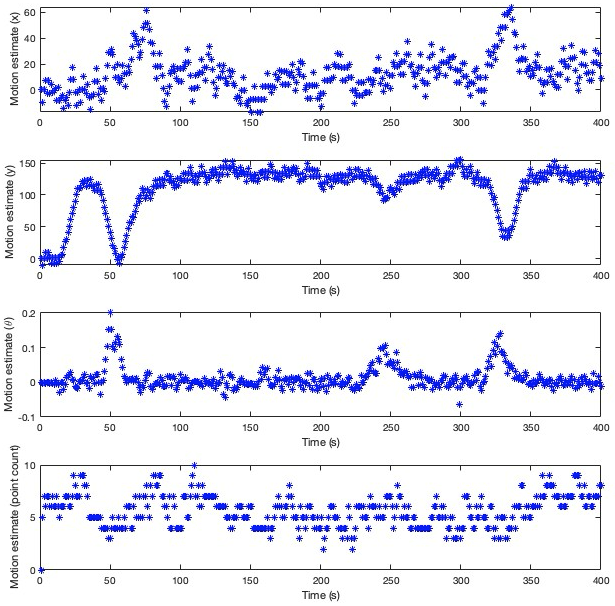
\includegraphics[width=0.8\linewidth, height=0.7\linewidth]{FastSLAM/Motion_Estimate.png}  
\caption{Motion Estimation Chart Over Time}
\label{fig:MotionEstimation}
\end{figure}
The motion path can be seen through Fig (\ref{fig:MotionPath}), which shows how the system is moving around and the map of the area it is moving around. \\
\begin{figure}[H]
  \centering
 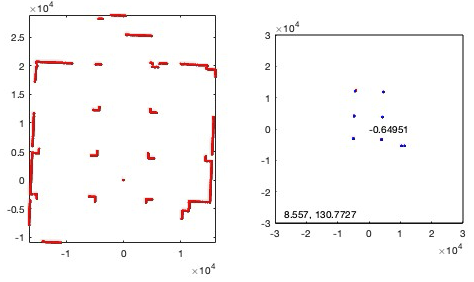
\includegraphics[width=0.7\linewidth, height=0.5\linewidth]{FastSLAM/Motion_Path.png}  
\caption{Actual Motion Path vs. Localized Estimated Path}
\label{fig:MotionPath}
\end{figure}

\textbf{Please explain what line 51-97  is trying to do?}\\
Lines 51-97 are associating the feature points P and Q based on their Mahalanobis distances. Where the Mahalanobis distance is a measure of the distance between a point and a distribution, taking into account the correlations of the data set and the shape of the distribution. This method allows the identification of corresponding features between P and Q detected corners, ensuring that only unique associations are taken as input while accounting for covariance in the measurements. The mahalanobis distance can be measured as:
\begin{equation}
D_M(\mathbf{x}, \boldsymbol{\mu}) = \sqrt{(\mathbf{x} - \boldsymbol{\mu})^T \Sigma^{-1} (\mathbf{x} - \boldsymbol{\mu})}
\label{EQ:DM}
\end{equation}
Where, \( D_M \): Mahalanobis distance between the point \( \mathbf{x} \) and the mean vector \( \boldsymbol{\mu} \). \( \mathbf{x} \): A point (vector) in the feature space for which the distance is being measured. \( \boldsymbol{\mu} \): Mean vector of the distribution (vector), representing the average position of all points in the dataset. \( \Sigma \): Covariance matrix of the distribution, representing the variance and covariance of the features in the dataset. \( T \): Transpose of the vector. \( \Sigma^{-1} \): Inverse of the covariance matrix.\\

A breakdown of the code can be shown below:
\begin{enumerate}
    \item Check for detected corners: check if there are any corners in 2nd set of corners and 1st set of corners (if either empty, then code block will be skipped)
    \begin{lstlisting}
    if (~isempty(corners2))
        if (~isempty(corners1))
    \end{lstlisting}
    \item Count the detected corners: \# of corners in corners1 and corners2
    \begin{lstlisting}
    known_corners_count = size(corners1, 2);
    detected_corners_count = size(corners2, 2);
    \end{lstlisting}
    \item Create the Mahalanobis distance Matrix: Create the matrix and initialize it to be "threshold" values. As the code iterates through, it will update this matrix with distance between pairs of detected corners
    \begin{lstlisting}
    mahalanobis_matrix = threshold.*ones(detected_corners_count, known_corners_count);
    \end{lstlisting}
    \item Calculate the Mahalanobis Distance: Iterate over each corner pair detected, and for each pair, calculate the difference in x-coordinate, y-coordinate, and angles (using slam in pi.m). Using Eq.(\ref{EQ:DM}) calculate the distance and store it into the matrix created above if it is less than the threshold values.
    \begin{lstlisting}
    for j = 1:detected_corners_count
        for k = 1:known_corners_count
		  % Components of x-mu
		  a = corners2(j).x-corners1(k).x;
		  b = corners2(j).y-corners1(k).y;
		  c = slam_in_pi(corners2(j).angle-corners1(k).angle);

		  mahalanobis_dist = sqrt([a b c] * (covariance^-1) * [a; b; c]);
		  if (mahalanobis_dist < threshold)
            mahalanobis_matrix(j,k) = mahalanobis_dist;
		  end
	   end
    end
    \end{lstlisting}
    \item Associating the points: find minimum distance within the mahalanobis matrix, if these distances are less than the threshold value, an association can be made and it finds the index of that value in the matrix and updates the associated count and stores them in the P and Q matrix. This continues to happen until associations can no longer be made, at which point the loop breaks.
    \begin{lstlisting}
while 1
    mahalanobis_min = min(min(mahalanobis_matrix));
    if (mahalanobis_min < threshold)
		% Associate, add to matrix of points
		[d_index, k_index] = find(mahalanobis_matrix == mahalanobis_min);
					
		if (size(d_index, 1) > 1)
			d_index = d_index(1);
		end
		if (size(k_index, 1) > 1)
			k_index = k_index(1);
		end
					
		assoc_count = assoc_count + 1;
		P(assoc_count,:) = [corners1(k_index).x corners1(k_index).y];
		Q(assoc_count,:) = [corners2(d_index).x corners2(d_index).y];
                    
		% Eliminate row and column from further consideration
		mahalanobis_matrix(d_index,:) = (threshold+1).*ones(1, known_corners_count);
		mahalanobis_matrix(:,k_index) = (threshold+1).*ones(detected_corners_count, 1);
	else
		break;
	end
end
    \end{lstlisting}
\end{enumerate}

\textbf{In the last part of the file (before plotting), what do you think is the advantage of constraining the change of x, y and theta?}\\
Constraining the change of x, y, and $\theta$ has many benefits such as enhancing the stability and accuracy of motion estimates, increasing the robustness of the system, and ensuring smoother trajectories through a less noisy system providing better navigation and mapping.\\

The system is more stable since constrained changes reduce the opportunity to destabilize the robot through fewer abrupt changes, which allows the UAV to navigate in a smoother manner while avoiding obstacles and following objects providing more stable and controlled navigation. \\

The system can provide more accurate motion estimates because the algorithm incorporates the estimated states of angle-pre and translation-pre, which improve the trajectory estimation as it takes into account the previous system state as well. \\

The system is more robust as a result of fewer measurement errors. Constrained values means that the noisy data from sensors from estimated position and orientation can be mitigated, reducing the impact of the errors on the system and providing a more accurate estimate for the system. \\

The UAV is able to achieve a smoother motion by preventing jumps in the position and orientation of the system and limiting changes to be within a specific threshold. This limiting can mitigate the noise or measurements that are outliers to affect the system and help provide a smoother motion estimate.\\

A constraint in the change of x,y, and $\theta$ also enforces smaller adjustments to the system from the sensors, which can reduce the over-corrections or oscillations that may occur in the position and orientation of the UAV due to sudden changes. This will also improve the association between frames through constrained changes, which increases the possibility of correctly matching features when the system is expecting smaller motion.\\

Finally, since the real world has several physical constraints on how quickly a robot can maneuver, we can use constraints to replicate practical scenarios to the best of our abilities and mimic real-world dynamics.